%%%%%%%%%%%%%%%%%%%%%%%%%%%%%%%%%%%%%%%%%
% Structured General Purpose Assignment
% LaTeX Template
%
% This template has been downloaded from:
% http://www.latextemplates.com
%
% Original author:
% Ted Pavlic (http://www.tedpavlic.com)
%
% Note:
% The \lipsum[#] commands throughout this template generate dummy text
% to fill the template out. These commands should all be removed when 
% writing assignment content.
%
%%%%%%%%%%%%%%%%%%%%%%%%%%%%%%%%%%%%%%%%%

%bias is close to zero because it is close to an unbiased estimator
%we would like to reduce the variance

%ridge regression: bias increases compared to other methods 
%as we increase alpha then the values drop

%naive bayes does not make i.i.d. assumption ONLY independance!

%for classification say which attributes are used i.e. say explicitly that the customer id will not be used 
%----------------------------------------------------------------------------------------
%	PACKAGES AND OTHER DOCUMENT CONFIGURATIONS
%----------------------------------------------------------------------------------------
\documentclass{Askarticle}
\usepackage[utf8]{inputenc}
\usepackage{fancyhdr} % Required for custom headers
\usepackage{lastpage} % Required to determine the last page for the footer
\usepackage{extramarks} % Required for headers and footers
\usepackage{graphicx} % Required to insert images
\usepackage{lipsum} % Used for inserting dummy 'Lorem ipsum' text into the template
\usepackage{amsmath}
\usepackage{amsfonts}
\usepackage{listings}
\usepackage{color}
%\usepackage{slashbox}
\usepackage{verbatim}
\usepackage{graphicx}

\usepackage{fancybox}
\usepackage{tikz}

 \usepackage[utf8]{inputenc}
\usepackage[english]{babel}
 
\usepackage{amsthm}
 
\usepackage[colorinlistoftodos]{todonotes}
\usepackage{algorithm}
\usepackage{algpseudocode}

\usepackage{color} %for colored boxes
\usepackage{empheq}

\usepackage{listings} %to include Code

\usepackage{geometry}
 \geometry{
 a4paper,
 total={210mm,297mm},
 left=20mm,
 right=20mm,
 top=20mm,
 bottom=20mm,
 }

%---------------------------------------------------------------------------------------------
%LISTINGS INITIAL
%---------------------------------------------------------------------------------------------
\definecolor{codegreen}{rgb}{0,0.6,0}
\definecolor{codegray}{rgb}{0.5,0.5,0.5}
\definecolor{codepurple}{rgb}{0.58,0,0.82}
\definecolor{backcolour}{rgb}{0.95,0.95,0.92}
\newcommand{\norm}[1]{\left\lVert#1\right\rVert}
 
\lstdefinestyle{mystyle}{
    backgroundcolor=\color{backcolour},   
    commentstyle=\color{codegreen},
    keywordstyle=\color{magenta},
    numberstyle=\tiny\color{codegray},
    stringstyle=\color{codepurple},
    basicstyle={\ttfamily \footnotesize},
    breakatwhitespace=false,         
    breaklines=true,                 
    captionpos=b,                    
    keepspaces=true,                 
    numbers=left,                    
    numbersep=5pt,                  
    showspaces=false,                
    showstringspaces=false,
    showtabs=false,                  
    tabsize=2
}
 
\lstset{style=mystyle}
%---------------------------------------------------------------------------------------------
% Margins
\topmargin=-0.45in
\evensidemargin=0in
\oddsidemargin=0in
\textwidth=6.5in
\textheight=9.0in
\headsep=0.25in 

\linespread{1.1} % Line spacing

% Set up the header and footer
\pagestyle{fancy}
%\lhead{\hmwkAuthorName} % Top left header
\rhead{\hmwkClass\ : \hmwkTitle} % Top center header
%\chead{\firstxmark} % Top right header
\lfoot{\lastxmark} % Bottom left footer
\cfoot{} % Bottom center footer
\rfoot{Page\ \thepage\ of\ \pageref{LastPage}} % Bottom right footer
\renewcommand\headrulewidth{0.4pt} % Size of the header rule
\renewcommand\footrulewidth{0.4pt} % Size of the footer rule

\setlength\parindent{0pt} % Removes all indentation from paragraphs

%----------------------------------------------------------------------------------------
%	DOCUMENT STRUCTURE COMMANDS
%	Skip this unless you know what you're doing
%----------------------------------------------------------------------------------------

% Header and footer for when a page split occurs within a problem environment
\newcommand{\enterProblemHeader}[1]{
\nobreak\extramarks{#1}{#1 continued on next page\ldots}\nobreak
\nobreak\extramarks{#1 (continued)}{#1 continued on next page\ldots}\nobreak
}

% Header and footer for when a page split occurs between problem environments
\newcommand{\exitProblemHeader}[1]{
\nobreak\extramarks{#1 (continued)}{#1 continued on next page\ldots}\nobreak
\nobreak\extramarks{#1}{}\nobreak
}

\setcounter{secnumdepth}{0} % Removes default section numbers
\newcounter{homeworkProblemCounter} % Creates a counter to keep track of the number of problems

\newcommand{\homeworkProblemName}{}
\newenvironment{homeworkProblem}[1][Problem \arabic{homeworkProblemCounter}]{ % Makes a new environment called homeworkProblem which takes 1 argument (custom name) but the default is "Problem #"
\stepcounter{homeworkProblemCounter} % Increase counter for number of problems
\renewcommand{\homeworkProblemName}{#1} % Assign \homeworkProblemName the name of the problem
\section{\homeworkProblemName} % Make a section in the document with the custom problem count
\enterProblemHeader{\homeworkProblemName} % Header and footer within the environment
}{
\exitProblemHeader{\homeworkProblemName} % Header and footer after the environment
}

\newcommand{\problemAnswer}[1]{ % Defines the problem answer command with the content as the only argument
\noindent\framebox[\columnwidth][c]{\begin{minipage}{0.98\columnwidth}#1\end{minipage}} % Makes the box around the problem answer and puts the content inside
}

\newcommand{\homeworkSectionName}{}
\newenvironment{homeworkSection}[1]{ % New environment for sections within homework problems, takes 1 argument - the name of the section
\renewcommand{\homeworkSectionName}{#1} % Assign \homeworkSectionName to the name of the section from the environment argument
\subsection{\homeworkSectionName} % Make a subsection with the custom name of the subsection
\enterProblemHeader{\homeworkProblemName\ [\homeworkSectionName]} % Header and footer within the environment
}{
\enterProblemHeader{\homeworkProblemName} % Header and footer after the environment
}
   
%----------------------------------------------------------------------------------------
%	NAME AND CLASS SECTION
%----------------------------------------------------------------------------------------
\newcommand\given[1][]{\:#1\vert\:} %define new command
\newcommand{\hmwkTitle}{Homework\ \#2} % Assignment title
\newcommand{\hmwkDueDate}{\today} % Due date
\newcommand{\hmwkClass}{TIM\ 245 - Data Mining} % Course/class
\newcommand{\hmwkClassTime}{4:20pm} % Class/lecture time
\newcommand{\hmwkClassInstructor}{Instructor: Tyler Munger} % Teacher/lecturer
\newcommand{\hmwkAuthorNameB}{Panos Karagiannis}
\newcommand{\hmwkOption}{Homework Heavy Option}
\newcommand{\hmwkIDA}{ID: -}

\newcommand{\Prb}{\mathbb{P}}
\newcommand{\N}{\mathcal{N}}
\newcommand{\R}{\mathbb{R}}
\newcommand{\E}{\mathbb{E}}
\newcommand{\answer}{\noindent\rule{16cm}{0.9pt}
		
		\large{\textbf{\underline{Answer:}}}

		\vspace{0.5cm}}
%----------------------------------------------------------------------------------------
%	TITLE PAGE
%----------------------------------------------------------------------------------------

\title{
\vspace{2in}
\textmd{\textbf{\hmwkClass:\ \hmwkTitle}}\\
\normalsize\vspace{0.1in}\small{Due:\ \textit{\hmwkDueDate}}\\
\vspace{0.1in}\large{\textit{\hmwkClassInstructor}}
\vspace{3in}
}

\author{\begin{tabular}{ l r }
					 \hmwkAuthorNameB \\
					\multicolumn{1}{c}{\hmwkIDA}
				\end{tabular}}
\date{} % Insert date here if you want it to appear below your name

%----------------------------------------------------------------------------------------

\begin{document}

\maketitle

%----------------------------------------------------------------------------------------
%	TABLE OF CONTENTS
%----------------------------------------------------------------------------------------

%\setcounter{tocdepth}{1} % Uncomment this line if you don't want subsections listed in the ToC

\newpage
\tableofcontents
\newpage

\newtheorem{theorem}{Theorem}
\newtheorem{panostheorem}{Theorem}
\newtheorem{claim}[theorem]{Claim}
\newtheorem{definition}[panostheorem]{Definition}

%----------------------------------------------------------------------------------------
%	BLUE BOX
%----------------------------------------------------------------------------------------



\definecolor{myblue}{rgb}{.8, .8, 1}



\newlength\mytemplen
\newsavebox\mytempbox

\makeatletter
\newcommand\mybluebox{%
    \@ifnextchar[%]
       {\@mybluebox}%
       {\@mybluebox[0pt]}}

\def\@mybluebox[#1]{%
    \@ifnextchar[%]
       {\@@mybluebox[#1]}%
       {\@@mybluebox[#1][0pt]}}

\def\@@mybluebox[#1][#2]#3{
    \sbox\mytempbox{#3}%
    \mytemplen\ht\mytempbox
    \advance\mytemplen #1\relax
    \ht\mytempbox\mytemplen
    \mytemplen\dp\mytempbox
    \advance\mytemplen #2\relax
    \dp\mytempbox\mytemplen
    \colorbox{myblue}{\hspace{1em}\usebox{\mytempbox}\hspace{1em}}}

\makeatother

%----------------------------------------------------------------------------------------
%	PROBLEM 1
%----------------------------------------------------------------------------------------

\begin{homeworkProblem}[Problem \arabic{homeworkProblemCounter}: Exploratory Analysis and Data Cleaning ]
Use a combination of visual and quantitative tools to answer the following questions for the five input attributes ($X$s) and the target ($Y$):

\begin{enumerate}
\item	What is the typical value (central tendency)?
\item What is the uncertainty (spread) for a typical value?
\item What is a good distributional fit for the data (symmetric, skewed, long-tailed)?
\item	Does the attribute affect other attributes (correlation)?
\item	Does the attribute contain outliers (extreme values)?

\end{enumerate}

It may be useful to format the answers as a table. Include any relevant plots and descriptive statistics in an appendix section.


\noindent\rule{16cm}{0.9pt}
		
\large{\textbf{\underline{Answer:}}}

After removing the column \texttt{name} from our dataset we have the following attributes: \\
\textbf{Xs} $\rightarrow$ \texttt{economy}, \texttt{family}, \texttt{health},  \texttt{freedom},  \texttt{government\_corruption} \\
\textbf{Y} $\rightarrow$ \texttt{happiness\_score} \\

For each of the aforementioned attributes follow the answers to Questions $1-5$:\\
\\ \texttt{economy}: 
\begin{enumerate}
\item \textsc{Typical Value}: Calculating the mean for this data using $R$ we get that the average is approximately $0.9539$
\item \textsc{Spread}: The standard deviation (sample) for this data is $0.4125954$. Also the mean absolute difference is $mad=0.43276$
\item \textsc{ Distributional fit}: Drawing a histogram of the data we see that the distribution looks \emph{relatively} symmetric around the mean.
\item  \textsc{Correlation}: The Pearson coefficient between \texttt{economy} and every other numerical attribute of this dataset is depicted in Table 1. We see that \texttt{economy} is most heavily correlated with family ($\sigma = 0.67$) and health ($\sigma=0.84$).
\item 	\textsc{Outliers}: Based on the histogram there does not seem to be significant outliers. Also, the standard deviation as well as the $mad$ are relatively small. 
\end{enumerate}

\texttt{family}: 
\begin{enumerate}
\item \textsc{Typical Value}: Calculating the mean for this data using $R$ we get that the average is approximately $0.7936$
\item \textsc{Spread}: The standard deviation (sample) for this data is $0.2667$. Also the mean absolute difference is $mad=0.2817$
\item \textsc{ Distributional fit}: Drawing a histogram of the data we see that the distribution looks skewed to the left. This means that there are few datapoints with small \texttt{family} values. 
\item  \textsc{Correlation}: The Pearson coefficient between \texttt{family} and every other numerical attribute of this dataset is depicted in Table 1. We see that \texttt{family} is most heavily correlated with economy ($\sigma = 0.67$) and \texttt{happiness\_score} ($\sigma=0.73$).
\item \textsc{Outliers}: Since the histogram is skewed there are outliers in this attribute. 
\end{enumerate}

\texttt{health}: 
\begin{enumerate}
\item \textsc{Typical Value}: Calculating the mean for this data using $R$ we get that the average is approximately $0.5576$
\item \textsc{Spread}: The standard deviation (sample) for this data is $0.2293$. Also the mean absolute difference is $mad=0.2478$
\item \textsc{ Distributional fit}: Drawing a histogram of the data we see that the distribution looks \emph{relatively} symmetric around the mean.
\item  \textsc{Correlation}: The Pearson coefficient between \texttt{health} and every other numerical attribute of this dataset is depicted in Table 1. We see that \texttt{health} is most heavily correlated with \texttt{economy} ($\sigma = 0.84$) and \texttt{happiness\_score} ($\sigma=0.77$).
\item \textsc{Outliers}: Even if the histogram is not skewed, we see that outliers do exist since the standard deviation as well as the $mad$ are large relative to the mean.
\end{enumerate}

\texttt{freedom}: 
\begin{enumerate}
\item \textsc{Typical Value}: Calculating the mean for this data using $R$ we get that the average is approximately $0.3710$
\item \textsc{Spread}: The standard deviation (sample) for this data is $0.1455$. Also the mean absolute difference is $mad=0.1662$
\item \textsc{ Distributional fit}: Drawing a histogram of the data we see that the distribution contains outliers. Therefore, this distribution is only  \emph{relatively} symmetric around the mean.
\item  \textsc{Correlation}: The Pearson coefficient between \texttt{health} and every other numerical attribute of this dataset is depicted in Table 1. We see that \texttt{freedom} is \textbf{not} heavily correlated with any other attribute. For example, it is most heavily correlated with \texttt{government\_corruption}  ($\sigma = 0.50$) and \texttt{happiness\_score} ($\sigma=0.57$).
\item \textsc{Outliers}: Based on the histogram for this data we see that outliers exist in the attribute. This is also reinforced by the fact that the standard deviation as well as the $mad$ are large relative to the typical value.
\end{enumerate}


\texttt{government\_corruption}:
\begin{enumerate}
\item \textsc{Typical Value}: Calculating the mean for this data using $R$ we get that the average is approximately $0.1376$
\item \textsc{Spread}: The standard deviation (sample) for this data is $0.1110$. Also the mean absolute difference is $mad=0.0792$
\item \textsc{ Distributional fit}: Drawing a histogram of the data we see that the distribution is very skewed to the right.
\item  \textsc{Correlation}: Based on Table 1 this attribute does not seem to be heavily correlated with any other attributes. It most heavily correlated with \texttt{freedom} and \texttt{happiness\_score}.
\item \textsc{Outliers}: Based on the histogram for this data we see that outliers exist in the attribute. This is also reinforced by the fact that the standard deviation as well as the $mad$ are large relative to the typical value.
\end{enumerate}

\texttt{happiness\_score}:
\begin{enumerate}
\item \textsc{Typical Value}: Calculating the mean for this data using $R$ we get that the average is approximately $5.382$
\item \textsc{Spread}: The standard deviation (sample) for this data is $1.141$. Also the mean absolute difference is $mad=1.371$
\item \textsc{ Distributional fit}: Drawing a histogram of the data we see that the distribution is \emph{relatively} symmetric around the mean.
\item  \textsc{Correlation}: Based on Table 1we see that \texttt{happiness\_score} is most heavily correlated with \texttt{economy} ($\sigma = 0.79$), \texttt{family} ($\sigma= 0.73$) and \texttt{health} ($\sigma= 0.77$).
\item \textsc{Outliers}: Based on the histogram for this data we see that outliers do not exist for the attribute. This is also becomes apparent from the fact that the standard deviation and the $mad$ are small compared to the mean. 
\end{enumerate}



\begin{table}[H]
		\caption{Upper Triangular Correlation Matrix}
		\centering
		\begin{tabular}{c c c c c c c}
		\hline\hline
		 {}&economy & family & health & freedom & government\_corruption & happiness\_score\\ [0.5ex] % inserts table %heading
		\hline
		economy & 1 & 0.67 & 0.84 & 0.36 & 0.29 &  0.79\\[0.1cm]  
		family &- & 1 & 0.59 & 0.45 & 0.21 & 0.73 \\ [0.1cm] 
		health &- & - & 1 & 0.34  & 0.25 & 0.77 \\ [0.1cm] 
		freedom &- & - & - & 1 & 0.50 & 0.57 \\ [0.1cm] 
		government\_corruption &- & - & - & - & 1 & 0.40 \\ [0.1cm] 
		happiness\_score &- & - & - & - & - & 1 \\ [0.1cm] 
		
		%\\ [1ex]
		\hline
		\end{tabular}\\[0.5cm]
		\label{table:nonlin}
\end{table}


$\implies$ \textsc{All histograms are included in the Appendix.}
\end{homeworkProblem}
% To have just one problem per page, simply put a \clearpage after each problem
%----------------------------------------------------------------------------------------
%	PROBLEM 2
%----------------------------------------------------------------------------------------

\begin{homeworkProblem}[Problem \arabic{homeworkProblemCounter}: Prediction]
Based on the results from the Exploratory Data Analysis, how well does the data-set fit the assumptions of linear regression? For example, is the data normally distributed?
	
\noindent\rule{16cm}{0.9pt}
		
\large{\textbf{\underline{Answer:}}}

By definition, linear regression attempts to estimate the type and strength of linear relationships in the training data set. Given our previous analysis, as well as the scatter plots we produced, we see that the \textbf{Xs} which have a strong linear relationship with \texttt{happiness\_score} ($Y$) are: \texttt{economy}, \texttt{family} and \texttt{health}. This is expected as these attributes have high correlation coefficients with \texttt{happiness\_score} i.e. $\sigma= 0.79, 0.73, 0.77$, respectively. Nevertheless, the attributes \texttt{freedom} and \texttt{government\_corruption} seem to not be linearly correlated with \texttt{happiness\_score}. \\


$\implies$ \textsc{All scatter plots are included in the Appendix.}
 \end{homeworkProblem}


%----------------------------------------------------------------------------------------
%	PROBLEM 3
%----------------------------------------------------------------------------------------
\begin{homeworkProblem}[Problem \arabic{homeworkProblemCounter}: Prediction]

What is the interpretation of the coefficients of the linear model? For example, which attributes have the strongest correlation with happiness? Does the model make sense?

\noindent\rule{16cm}{0.9pt}
		
\large{\textbf{\underline{Answer:}}}

When we compile the model using the command:
\[ \texttt{fit.lm(happiness\_score)~.,data =train)} \]
 we get the following best fit straight line:
 \[ 
	happiness\_score = 
 \begin{bmatrix}\beta_{0} & \beta_{1} & \beta_{2} & \beta_{3} & \beta_{4}& \beta_{5}\end{bmatrix}\\
  \begin{bmatrix}1\\ economy \\ family \\ health \\ freedom \\ government\_corruption  \end{bmatrix}
 \]
 
 Since we are taking a random sample in order to test our data we see that every time we run the above command we get quite different results. For example:
\[ 
	happiness\_score = 
 \begin{bmatrix}2.208& 0.604 & 1.22 & 1.596 & 1.64 & 0.91\end{bmatrix}\\
  \begin{bmatrix} 1\\economy \\ family \\ health \\ freedom \\ government\_corruption \end{bmatrix}
 \]
 \[ 
	happiness\_score = 
 \begin{bmatrix}2.352&0.769 & 0.881 & 1.767 & 1.150 & 1.04\end{bmatrix}\\
  \begin{bmatrix} 1\\ economy \\ family \\ health \\ freedom \\ government\_corruption  \end{bmatrix}
 \]
 
 ,are both results given by our regression model but for different samples. This might be because of the fact that we are only training on $66\%$ of the total data ($\sim$ $100$ data points). Hence, there is a lot of variability in choosing our sample. \\
 
 The coefficients indicate the strength and type of the relationship. Firstly, we see that all coefficient are positive which is expected based on the correlation matrix (Table 1). \\
 
 Moreover, the greater the magnitude of a coefficient, the greater the correlation between the corresponding attribute and the dependent variable. In this model we see that \texttt{government\_corruption} has a small coefficient which is expected since as we discussed earlier this attribute has a very small correlation with \texttt{happiness\_score}. Nevertheless, based on our previous analysis we would expect the coefficient of \texttt{economy} to be much larger than the coefficient of \texttt{freedom} because the latter is very weakly correlated to \texttt{happiness\_score}. \\
 
 Finally, based on the magnitude of the coefficients we see that the attributes that have the strongest correlation to happiness are: \texttt{freedom}, \texttt{health}, \texttt{family}.

\end{homeworkProblem}
%----------------------------------------------------------------------------------------
%	PROBLEM 4
%----------------------------------------------------------------------------------------
\begin{homeworkProblem}[Problem \arabic{homeworkProblemCounter}: Prediction]
Provide an assessment of the model's performance. Do you think the model's performance is good? Explain why.

\noindent\rule{16cm}{0.9pt}
		
\large{\textbf{\underline{Answer:}}}

Using $R$ we get that $MSE= 0.32$ while the minimum and maximum value are $3.592$ and $7.355$, respectively. This signifies that the predicted value is not very inaccurate since the $MSE$ is small compared to the values of the coefficients. This is also reinforced by the fact that $RAE$ is small ($0.08$). Moreover in order to create a baseline for our model, we create a simple linear regression model where we use only one attributes and pick then pick the model with the minimum \emph{MSE}. In this case we choose the attribute \texttt{economy}, whose $MSE=0.46$. Therefore, we see that our model performs better than the baseline.

\newpage
		
\end{homeworkProblem}

%----------------------------------------------------------------------------------------
%	PROBLEM 5
%----------------------------------------------------------------------------------------
\begin{homeworkProblem}[Problem \arabic{homeworkProblemCounter}: Prediction]
How are the coefficients different for the linear model created using lm()? .Experiment with lambda values: $0.0005, 0.005, 0.5, and 5$. How do the coefficients change as we adjust the value of lambda up and down? 

\noindent\rule{16cm}{0.9pt}
		
\large{\textbf{\underline{Answer:}}}

As expected, when we use the more sophisticated linear regression methods the coefficients' magnitude decreases compared to the simple \texttt{lm()} method. This is logical since \emph{lasso, ridge and elastic nets} all use regularization methods because their loss function penalizes the magnitude of the coefficients. As we increase the parameter $\alpha$ the general trend is that the magnitude of the coefficients decreases more and more. For example the coefficient of \texttt{economy} becomes: $0.6195772, 0.6193755, 0.5958423, 0.5958423$ for $\alpha=0.0005, 0.005, 0.5, 5$, respectively.



\end{homeworkProblem}

%----------------------------------------------------------------------------------------
%	PROBLEM 6
%----------------------------------------------------------------------------------------
\begin{homeworkProblem}[Problem \arabic{homeworkProblemCounter}: Prediction]
Which model would you recommend to a nation that is trying to predict the happiness of their citizens?

\noindent\rule{16cm}{0.9pt}
		
\large{\textbf{\underline{Answer:}}}

The model that I would suggest in predicting the happiness of the citizens would be the \emph{elastic net} model. \emph{Elastic net} is a hybrid model that uses parts from both lasso and ridge regression. By combining both the $L1$ and $L2$ norm in the penalty function, \emph{elastic net} could give promising results. This is also reinforced by the fact that the $MSE$ for \emph{elastic net} is $0.3512$ ,whereas, for \emph{lasso} and \emph{ridge} the $MSE$ is $0.3524, 0.3522$, respectively. 

\end{homeworkProblem}


%----------------------------------------------------------------------------------------
%	PROBLEM 7
%----------------------------------------------------------------------------------------
\begin{homeworkProblem}[Problem \arabic{homeworkProblemCounter}: Prediction]
What is the interpretation of the selected model? What can we say about the relationship between the input attributes and the happiness score? \\

\textbf{Extra Credit:}

Show that $coef(lm(\mathbf{Y} \sim \mathbf{X})) $ is equivalent to $\hat{\boldsymbol{\beta}}= (\boldsymbol{X}^{T} \boldsymbol{X})^{-1} \boldsymbol{X}^{T}\boldsymbol{Y}$

\noindent\rule{16cm}{0.9pt}
		
\large{\textbf{\underline{Answer:}}}

The model that we have created can be used to predict the happiness of people based on $6$ predefined attributes. The coefficients of our model tell us the mean change in the response variable (\emph{happiness}), for one unit of change in the predictor variable while holding other predictors in the model constant. Moreover, the $y-$ intercept in our model is approximately $2.35$ which signifies the baseline happiness i.e. when all other factors are $0$. \\


\textbf{Extra Credit:}\\
We prove this mathematically. Let $\boldsymbol{Y} \in \mathbb{R}^{n}, \boldsymbol{X }\in  \mathbb{R}^{n\times k}$, $\boldsymbol{\beta}\in  \mathbb{R}^{k}$.  Then, in the context of linear regression, we need to find the coefficients $\boldsymbol{\beta}$ that minimize our error function. In this case let the error function be $\mathcal{L}: \mathbb{R}^{n} \rightarrow \mathbb{R} $ with formula:

\[ \mathcal{L}(\boldsymbol{\beta}) = \norm {\boldsymbol{Y}- \boldsymbol{X}\boldsymbol{\beta} }^2 = 
(\boldsymbol{Y}- \boldsymbol{X}\boldsymbol{\beta})^{T})(\boldsymbol{Y}- \boldsymbol{X}\boldsymbol{\beta} )   \]

Our objective is to minimize the loss w.r.t. $\boldsymbol{\beta}$ hence we need to find $\hat{\boldsymbol{\beta}}$ such that $\mathcal{L}$ is minimum. 

Before taking the derivative we expand the expression for the loss: 
\begin{align}
  (\boldsymbol{Y}- \boldsymbol{X}\boldsymbol{\beta})^{T})(\boldsymbol{Y}- \boldsymbol{X}\boldsymbol{\beta} )  =\\
\boldsymbol{Y}^{T}\boldsymbol{Y}-  (\boldsymbol{X}\boldsymbol{\beta})^{T} \boldsymbol{Y} - \boldsymbol{Y}^{T} \boldsymbol{X}\boldsymbol{\beta} - (\boldsymbol{X}\boldsymbol{\beta})^{T}\boldsymbol{X}\boldsymbol{\beta}= \\
\boldsymbol{Y}^{T}\boldsymbol{Y}-2\boldsymbol{Y}^{T} \boldsymbol{X}\boldsymbol{\beta} - \boldsymbol{\beta}^{T}\boldsymbol{X}^{T}\boldsymbol{\beta}\boldsymbol{X}
\end{align}

In order to compute the derivative of (3) we need to show the following results: \\

Let $f(\boldsymbol{\beta})= \boldsymbol{c}^{T} \boldsymbol{\beta}$. Then: 
\[f= \sum_{i=1}^{k} c_{i}\beta_{i} \]
Hence: 
\[ \frac{\partial f} {\partial \beta_{w}}= \sum_{i=1}^{k} c_{i} \frac{\partial  \beta_{i}} {\partial \beta_{w}} = c_{w}  \]
So: 
\begin{align}
\nabla_{\boldsymbol{\beta} } f = \boldsymbol{c}
\end{align}

Now let the more interesting function $ f(\boldsymbol{\beta})= \boldsymbol{\beta}^{T} \boldsymbol{A}\boldsymbol{\beta}$, for $A$ k-dimensional square matrix. Then:

\[  f= \sum_{i=1}^{k} \sum_{j=1}^{k} \alpha_{ij} \beta_{i} \beta_{j} =  \]

Differentiating this expression we get:

\begin{align*}
 \frac{\partial f} {\partial \beta_{w}}= \sum_{i=1}^{k} \sum_{j=1}^{k} \alpha_{ij} \frac { \partial (\beta_{i} \beta_{j})  } {\partial \beta_{w}} =
\sum_{i=1}^{k} \sum_{j=1}^{k} \alpha_{ij} ( \delta_{i,w} \beta_{j} + \delta_{j,w}\beta_{i} )= \\
 \sum_{j=1}^{k} \alpha_{wj} \beta_{j} +  \sum_{i=1}^{k} \alpha_{iw} \beta_{i} = (\boldsymbol{A} \boldsymbol{\beta} )_{w} +  \sum_{i=1}^{k} (\boldsymbol{A})^{T}_{w,i} \, \beta_{i}= (\boldsymbol{A} \boldsymbol{\beta} )_{w} + (\boldsymbol{A}^{T} \boldsymbol{\beta} )_{w}
 \end{align*}
 
 Hence we gey that:
\begin{align}
\nabla_{\boldsymbol{\beta} } f = (\boldsymbol{A+A^{T}}) \boldsymbol{\beta}
\end{align}

Finally, we are in place to differentiate $(3)$ using $(4),(5)$. Let $\boldsymbol{Y}^{T} \boldsymbol{X} = \boldsymbol{c}$ and also let $\boldsymbol{X}^{T}\boldsymbol{X}=\boldsymbol{A}$ . Then we get:

\begin{align}
\nabla_{\boldsymbol{\beta}} \mathcal{L}= \boldsymbol{0} - 2 \boldsymbol{Y}^{T} \boldsymbol{X} + (\boldsymbol{X}^{T}\boldsymbol{X} +(\boldsymbol{X}^{T}\boldsymbol{X})^{T} ) \boldsymbol{\beta}= \\
-2 \boldsymbol{Y}^{T} \boldsymbol{X} + 2\boldsymbol{X}^{T}\boldsymbol{X} \boldsymbol{\beta}= 2(\boldsymbol{X}^{T}\boldsymbol{X} \boldsymbol{\beta} -  \boldsymbol{Y}^{T} \boldsymbol{X}   )
\end{align}


Equating the derivative with $\mathbf{0}$ and solving the equation we get  $\hat{\boldsymbol{\beta}}$:

\[\boldsymbol{X}^{T} \boldsymbol{X} \hat{\boldsymbol{\beta}}-\boldsymbol{X}^{T}\boldsymbol{Y} =\mathbf{0}  \iff  
 \boldsymbol{X}^{T} \boldsymbol{X} \hat{\boldsymbol{\beta}}- \boldsymbol{X}^{T}\boldsymbol{Y}=\mathbf{0}  \iff \]


\[  \iff \boldsymbol{X}^{T} \boldsymbol{X} \hat{\boldsymbol{\beta}} = \boldsymbol{X}^{T}\boldsymbol{Y} \iff 
	\hat{\boldsymbol{\beta}}= (\boldsymbol{X}^{T} \boldsymbol{X})^{-1} \boldsymbol{X}^{T}\boldsymbol{Y} 
\]

To verify these results experimentally is straighforward. We use \texttt{X<-data.matrix(data[0:5])} and then set the first column to be $1$'s to define
 $\boldsymbol{X}$. Then, do  \texttt{Y<-data.matrix(data[6])} to set table $\boldsymbol{Y}$. To compute the transpose we do \texttt{X\_T<-t(X)}, whereas the inverse of the product is computed using \texttt{ solve( X\_T \%*\% X) }. Putting everything together we get: 

\[ \texttt{  b\_hat= solve( X\_T \%*\% X) \%*\% X\_T  \%*\% Y } \]
\vspace{15pt}
\end{homeworkProblem}


\textbf{In the following classification problems, we filter out the costumer id since it explodes our feature space and does not contribute to our classification procedure.} \\

\begin{homeworkProblem}[Problem 1: Classification]
How does the ZeroR model work? How is the ZeroR useful when creating a baseline?

\noindent\rule{16cm}{0.9pt}
		
\large{\textbf{\underline{Answer:}}}

The ZeroR model is one of the simplest ways to perform classification. In this classifier, we completely ignore the attributes and we simply always predict the majority class. Due to its simplicity and ease of implementation it is often used as a benchmark for other classification methods. \\

Using 10-fold cross validation in our example, we see that by using ZeroR we classify correctly $73.463\%$ percent of the instances. Moreover, the $F$ measure is $0.622$

\end{homeworkProblem}


\begin{homeworkProblem}[Problem 2: Classification]
Compare and contrast the performance of the three models. Do the Naive Bayes and Decision Tree models significantly outperform the ZeroR model? Explain why or why not.

\noindent\rule{16cm}{0.9pt}
		
\large{\textbf{\underline{Answer:}}}

When we compute the \emph{ Naive Bayes} we get a bit worse accuracy but better $F$-measure results than the ZeroR method (Accuracy=$71.9296\%$, $F=0.735$). Therefore, we see that Naive Bayes does not significantly outperform our baseline. One reason for this result, might be the independence assumptions that Naive Bayes makes to compute the posterior distribution. It is very likely that the attributes of our datasets are highly correlated therefore Naive Bayes performs poorly.\\

When we use \emph{Decision Trees} we get that the accuracy is $77.9781\%$, whereas, the $F$ measure is $0.772$. As a result we see that this method outperforms both $ZeroR$ as well as \emph{ Naive Bayes}. A possible reason for this result, might be the fact that Decision Trees do not make any independence assumptions (as in Naive Bayes) and also do not ignore the attributes (as in ZeroR).


\end{homeworkProblem}


\begin{homeworkProblem}[Problem 3: Classification]
How does the performance of the K-NN model compare to the baseline models from Experiment 1? 

\noindent\rule{16cm}{0.9pt}
		
\large{\textbf{\underline{Answer:}}}

Using the \emph{K-NN} method with $K=10$ we see it surpasses all methods used in previous questions in terms of both accuracy and $F$ measure, except  the \emph{Decision Trees}. More precisely, the accuracy we get for \emph{K-NN} is $77.5806\%$ whereas the $F$-measure is $0.767$.

\end{homeworkProblem}




\begin{homeworkProblem}[Problem 4: Classification]
Should the input attributes be normalized? Explain why or why not.
 

\noindent\rule{16cm}{0.9pt}
		
\large{\textbf{\underline{Answer:}}}

The attributes should definitely be normalized. For instance, the \texttt{Total Charges} are in the range of $[0,10^{3}]$ whereas \texttt{tenure} ranges from $[0, 10^2]$. Since we used the Euclidean distance in our model, the term differences of the \texttt{Total Charges} would dominate the sum. As a result, the ``effect'' of the \texttt{tenure} in our model would be diminished. 

\end{homeworkProblem}



\begin{homeworkProblem}[Problem 5: Classification]
Experiment with the following values for K=3,10,50,100. What effect does changing K have on the model performance? What is the optimal value for K? Explain why.

\noindent\rule{16cm}{0.9pt}
		
\large{\textbf{\underline{Answer:}}}

We see that as we increase the value of $K$ our results keep getting more accurate up to a point and then start getting more inaccurate. This fact is attributed to overfitting our test data. Below follow the measures we get as we increase $K$: 
\begin{enumerate}
\item $K=1$: Accuracy=$71.4894\%$ , $F$-measure=$0.717$
\item $K=10$: Accuracy=$77.5806\%$ , $F$-measure=$0.767$
\item $K=50$: Accuracy=$79.3554\%$ , $F$-measure=$0.791$ 
\item $K=100$: Accuracy=$79.327\%$ , $F$-measure=$0.790$ 
\end{enumerate}

As we increase $K$, both the accuracy as well as the $F$-measure get better, nevertheless, when $K$ reaches $100$ we have \textbf{overfitted} the data therefore our results become worse. From the above list, the optimal value of $K$ is $50$ (given these results, above we could also do a binary search to find the optimal $K$ in logarithmic time).
\end{homeworkProblem}


\begin{homeworkProblem}[Problem 6: Classification]
Compare and contrast the linear models (Logistic Regression and SVM) to the baseline and the non-linear models from the previous experiments? 

\noindent\rule{16cm}{0.9pt}
		
\large{\textbf{\underline{Answer:}}}

Both models \emph{Logistic Regression} and \emph{SVM} as discriminative methods therefore they do not make any underlying assumptions for the distribution of the data points and also minimize a loss function in order to find the optimal weights. This means that we would expect them to outperform the previously used methods. Running these tests in $Weka$ we see the following results:
\begin{enumerate}
\item $Logistic$: Accuracy=$80.2215\%$, $F$-measure=$0.809$
\item $SVM$: Accuracy=$80.2641\%$, $F$-measure=$0.810$

\end{enumerate}

\end{homeworkProblem}


\begin{homeworkProblem}[Problem 7: Classification]
Which model performs better: logistic regression or SVM? If there is a difference, explain why.

\noindent\rule{16cm}{0.9pt}
		
\large{\textbf{\underline{Answer:}}}

Both models behave very similarly, but we see that the $SVM$ model slightly outperforms \emph{Logistic Regression}. Both these methods minimize convex loss functions and hence any local minimum is also guaranteed to be a global minimum as well. The reason that the $SVM$ has a bit better accuracy is because it uses the \emph{hinge} loss which punishes misclassification, whereas, the logarithmic loss (used in Logistic Regression) leads at better probability estimation at the cost of accuracy.

\end{homeworkProblem}

\begin{homeworkProblem}[Problem 8: Classification]
Compare and contrast the Random Forest model with the results from Experiments 1, 2, and 3.

\noindent\rule{16cm}{0.9pt}
		
\large{\textbf{\underline{Answer:}}}

Running the \emph{Random Forest} model in Weka we get the following results: Accuracy=$77.4790\%$ and $F$-measure= $0.763$. The idea behind a Random Forest is the use of many Decision Trees to classify a given vector. Therefore, this model is very similar to Decision Trees and does not make any assumptions about the underlying distribution of the data points as in Naive Bayes. We see that the \emph{Random Forest} outperforms \emph{ZeroR} and \emph{Naive} Bayes, nevertheless, has very similar results to \emph{Decision Trees}. \\

Moreover, comparing \emph{KNN} with \emph{Random Forest} depends on the value of the parameter $K$ that we choose for our \emph{KNN} model. For $K<10$, we observe that \emph{Random Forest} outperforms \emph{KNN}, whereas, the opposite happens when $10 \leq K \leq 100$.\\

Finally, we see that both \emph{Logistic Regression} as well as \emph{SVM} outperform \emph{Random Forest}. This might be due to the power of the methods used in Problem $3$ in minimizing a loss function to find the optimal weights.

\end{homeworkProblem}

\begin{homeworkProblem}[Problem 9: Classification]
What is the difference between a Random Forest and the decision tree model from Experiment 1. Would you expect the Random Forest model to outperform the decision tree model? Explain why.

\noindent\rule{16cm}{0.9pt}
		
\large{\textbf{\underline{Answer:}}}

We would expect that the Random Forest would outperform the Decision Trees since in the former model we operate by constructing a multitude of decision trees at training time and outputting the class that is the mode of the classes. Nevertheless, this is not verified by our experimental results. As we observe, both models perform very similarly in both their Accuracy as well as their $F$-measure. This observation might be because during the \emph{Random Forest} model we generate many \emph{Decision Trees} which only ``mislead'' us and introduce noise to the final decision.

\end{homeworkProblem}

\begin{homeworkProblem}[Problem 10: Classification]
What model do you recommend that the telecommunications company use to predict churn? Explain why.



\noindent\rule{16cm}{0.9pt}
		
\large{\textbf{\underline{Answer:}}}

The model I would suggest to the telecommunications company to use in order to predict churn would be \emph{SVM}. There are two basic reasons as to why I would suggest the $SVM$ model against any other model considered in this assignement. \\

Firstly, as we saw experimentally the $SVM$ outperforms most of the models that we used, in both accuracy and $F$-measure. This is mainly because it is not forced to make any assumptions about how the data were distributed or generated. Solving a loss function to minimize the margin is a powerful technique that inevitably yields good results. \\ 

Secondly, the true power of $SVMs$ becomes apparent when the telecommunications company would like to incorporate much more features (attributes) into their model. Then instead of solving the \emph{Primal Problem} we can equivalently solve the \emph{Dual Problem}. \\

For example let the dimension of our attributes be $D$. Then solving the Primal problem would be much more inefficient in the case where $D \gg N$. This is obvious from the formulas of the two equivalent problems: 
	\begin{equation*}
		\begin{aligned}
		&\textbf{Primal:} \\
		& \underset{w,b}{\text{minimize}}
		& &  \frac{1}{2} \| \mathbf{w}\|  + \frac{C}{M} \sum_{i=0}^{M} \xi_i  \\
		& \text{subject to}
		& & t_i ( <\mathbf{w}, x_i> +b) \geq 1 - \xi_i \\
		& & & \xi_i \geq0
		\end{aligned}
		\end{equation*}

	In the Primal we see that we optimize over $\mathbf{w}$ which is a D-dimensional vector. Therefore if the feature space is large, then it 
	would imply large complexity in solving the above problem. On the contrary, by manipulating the Lagrangian we obtain the formula for the Dual:
		\begin{equation*}
		\begin{aligned}
		&\textbf{Dual:} \\
		& \underset{\alpha}{\text{minimize}}
		& &  \alpha^T H \alpha - \alpha^T e \\
		& \text{subject to}
		& & \alpha^T \mathbf{t} =0 \\
		& & &0 \leq \alpha \leq \frac{C}{M}
		\end{aligned}
		\end{equation*}
		
	Which is a minimization over the N-dimensional vector $\alpha$. This means that now our problem only depends on the number 	of data points. Moreover in order to retrieve $\mathbf{w}$ we can calculate:  
	\[  \mathbf{w}= \sum_{i=0}^{M} \alpha_i t_i x_i\]
	But that still would very inefficient since we would have to store and maintain a D-dimensional vector. Instead we can use kernel 
	functions to overcome this barrier. If we let $K$ be the kernel associated with the RKHS we can say that: 
	\[  < \mathbf{w}, x> = \sum_{i=0}^{M} \alpha_i t_i K(x_i,x)\]
	To further illustrate why the Dual is often more efficient, consider the example of classification of emails. Then let  $\mathbf{x}_i$ be the binary 	vector containing information on whether an email contains word $i$. Then if we attempt to incorporate bigrams and trigrams in in our 
	vector $\mathbf{x}_i$ we see that the dimension $D$ grows exponentially. Therefore, representing richer and richer concepts in our 
	vector explodes the complexity in the Primal space.\\
	
	 As a result, by using $SVMs$  the telecommunications company would be able to incorporate more and more attributes, or even combinations of attributes without facing any optimization problems.
	
	
	

\end{homeworkProblem}

\newpage
\begin{homeworkProblem}[Problem 11: Classification]
What are the limitations of the recommended model? How do you recommend that it be used? 

\noindent\rule{16cm}{0.9pt}
		
\large{\textbf{\underline{Answer:}}}

Even though $SVMs$ have many limitations, I think that the most significant one is that of overfitting. In general is it true that kernel models are more sensitive than other models in terms of overfitting. Therefore, the telecommunications company would have to be careful in their choice of parameters of the model. \\

A possible use of this prediction model would be to create specific favorable policies for customers who are about to churn. That way, the telecommunications company would be able to maintain more customers and as a result increase its profits.

\end{homeworkProblem}




%----------------------------------------------------------------------------------------
%	Appendix
%----------------------------------------------------------------------------------------
\begin{homeworkProblem}[Appendix]
\begin{figure}[htp]

\centering
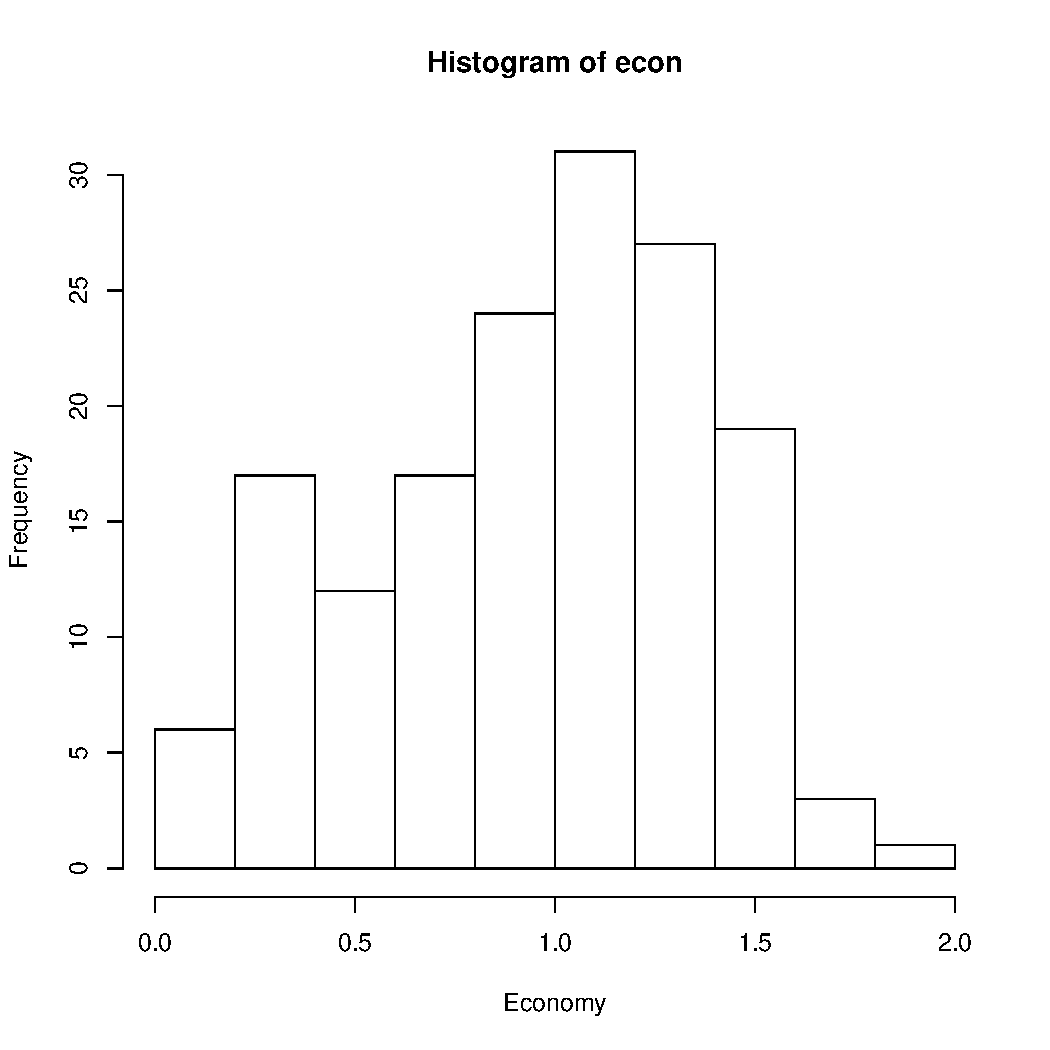
\includegraphics[width=.45\textwidth]{econ_hist.pdf}\hfill
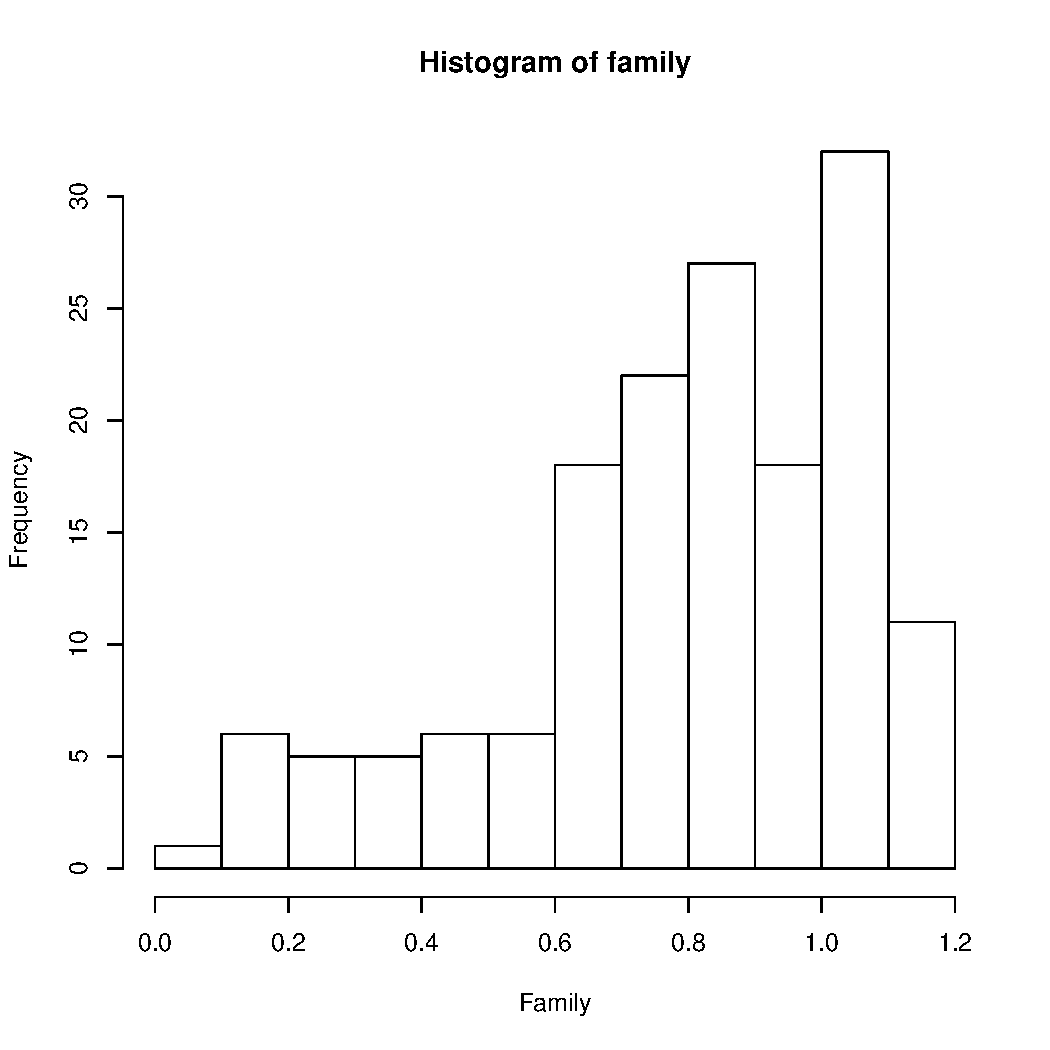
\includegraphics[width=.45\textwidth]{fam_hist.pdf}\hfill
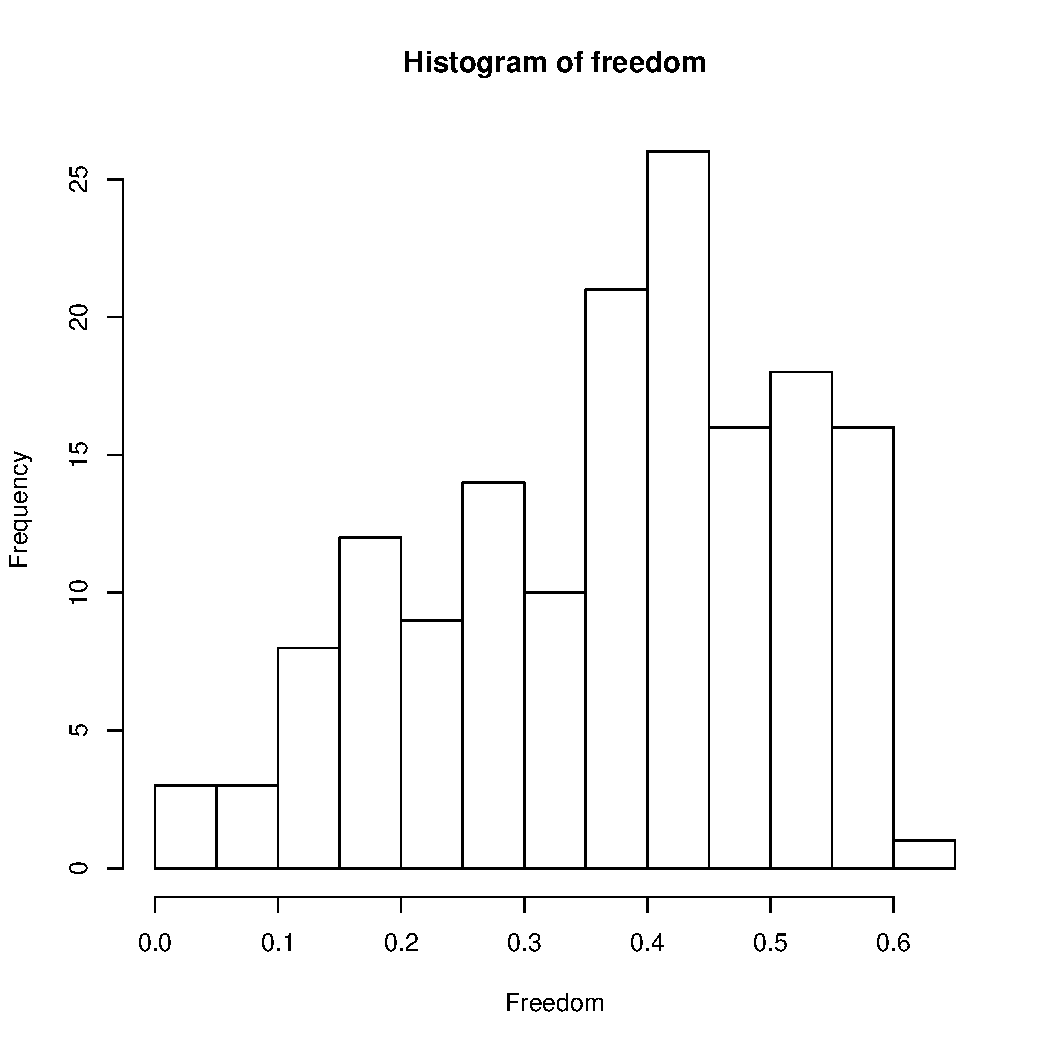
\includegraphics[width=.45\textwidth]{free_hist.pdf}\hfill
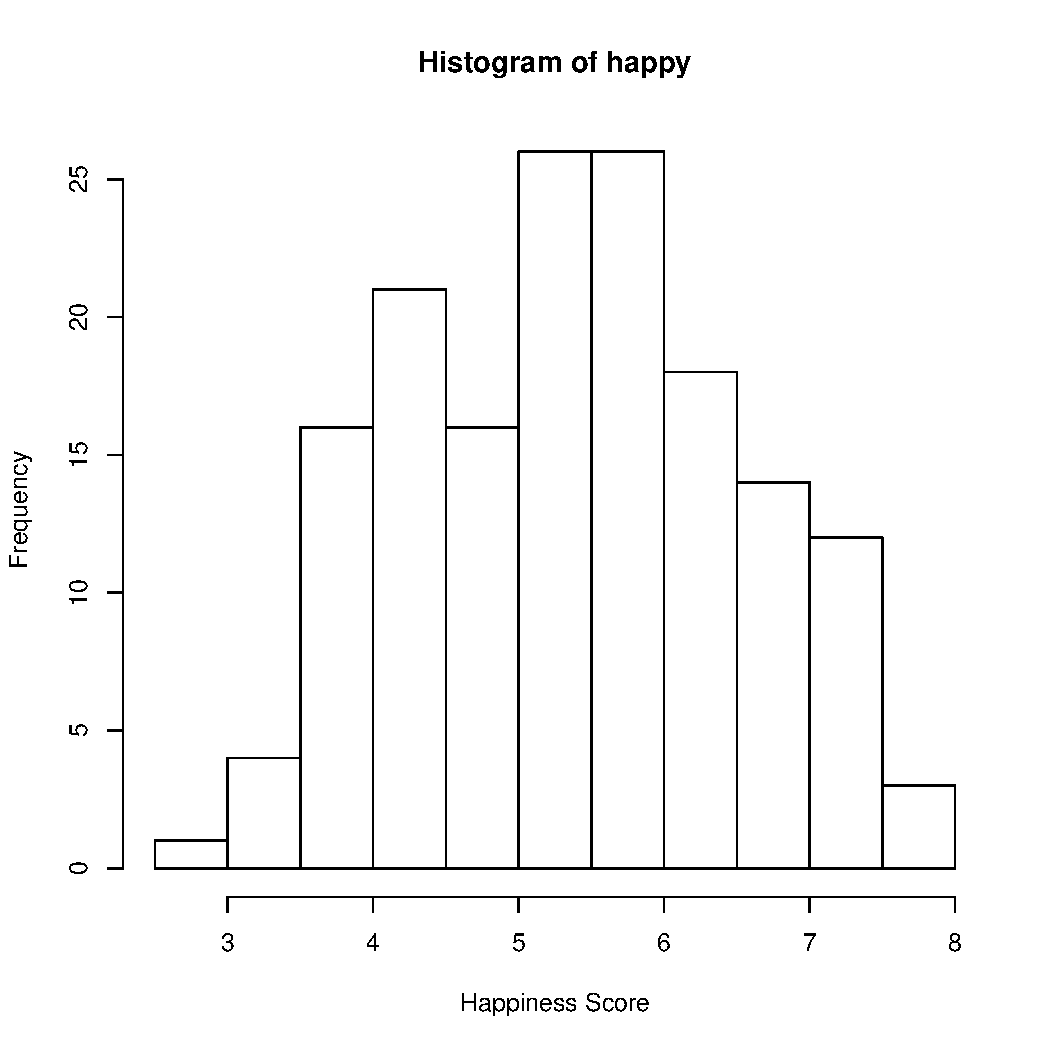
\includegraphics[width=.45\textwidth]{happy_hist.pdf}\hfill
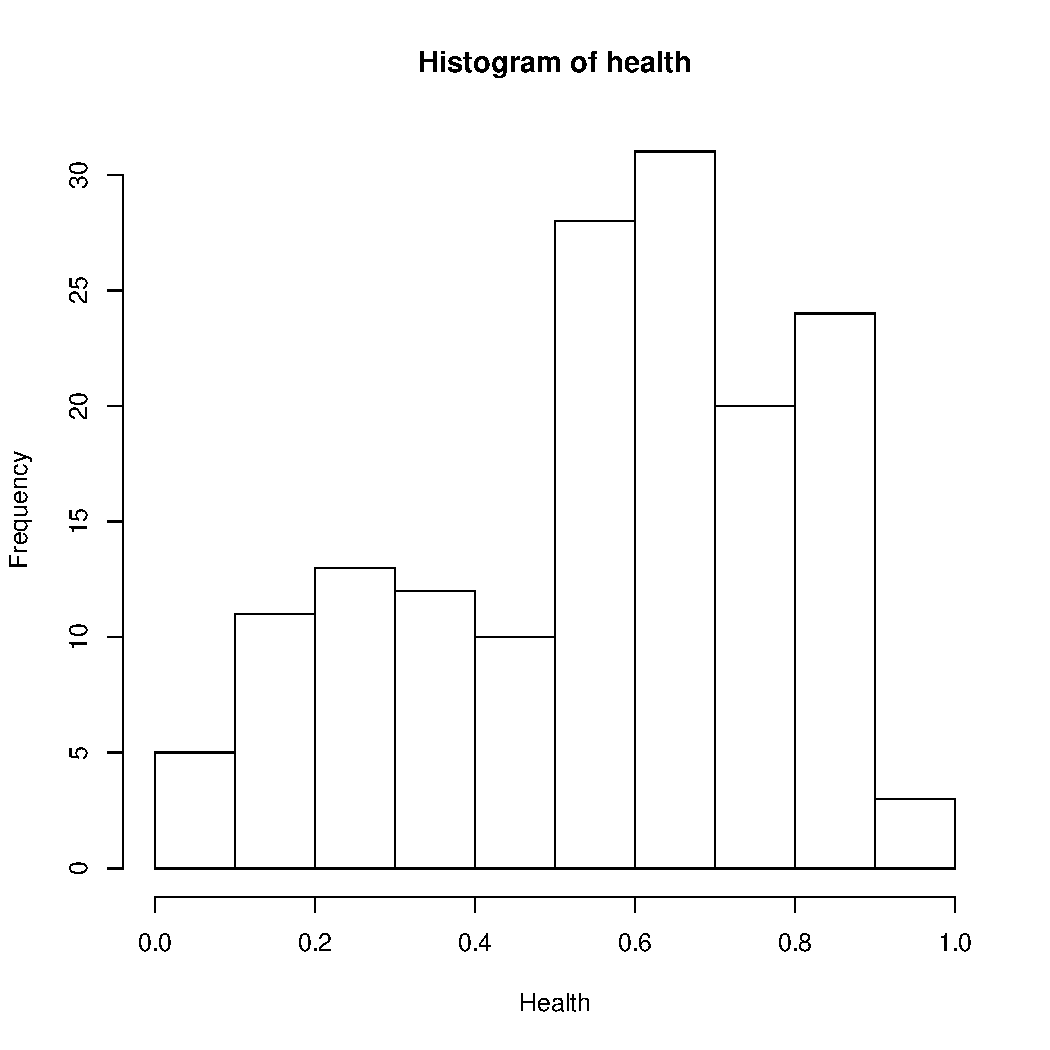
\includegraphics[width=.45\textwidth]{health_hist.pdf}\hfill
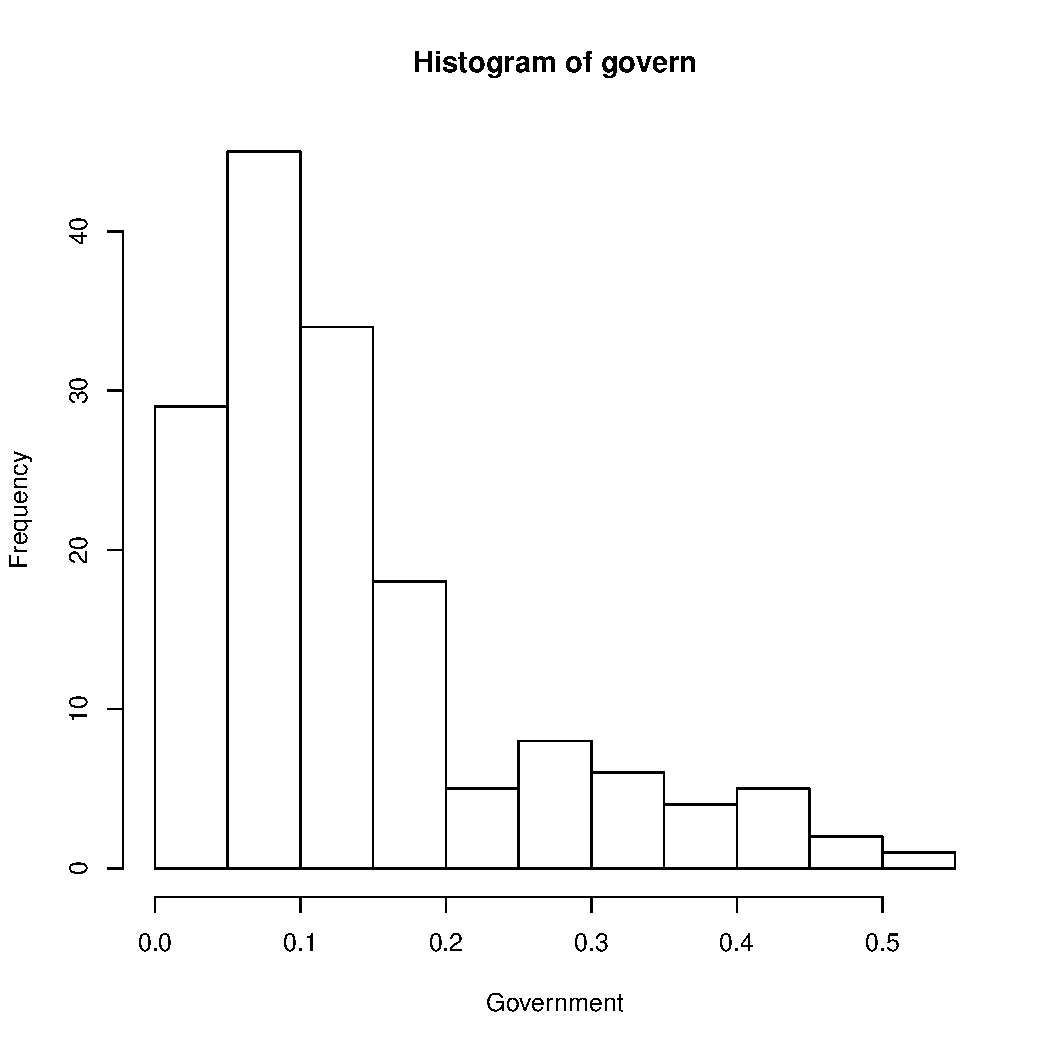
\includegraphics[width=.45\textwidth]{gov_hist.pdf}\hfill

\caption{Histograms for all the given variables}
\label{fig:figure3}

\end{figure}

\begin{figure}[htp]

\centering
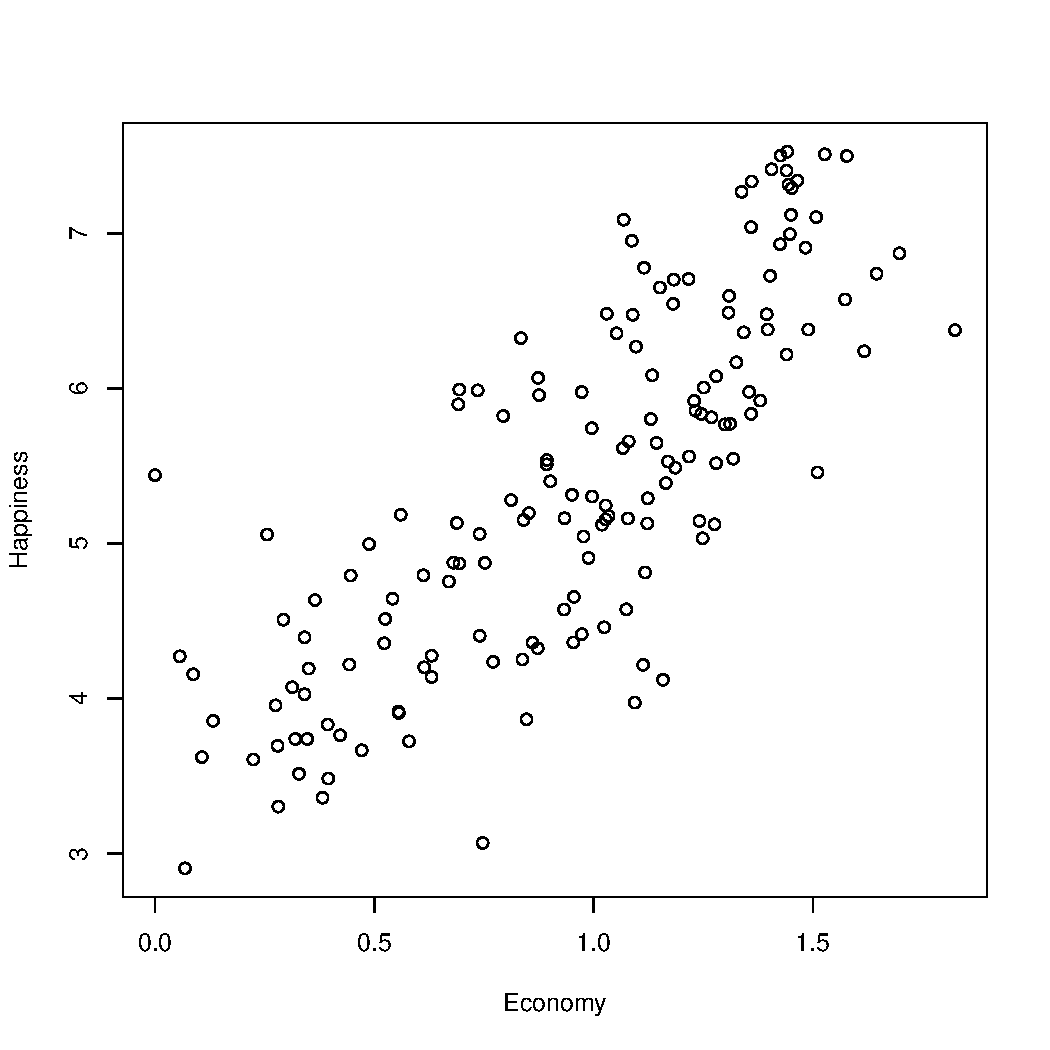
\includegraphics[width=.45\textwidth]{econ_plot.pdf}\hfill
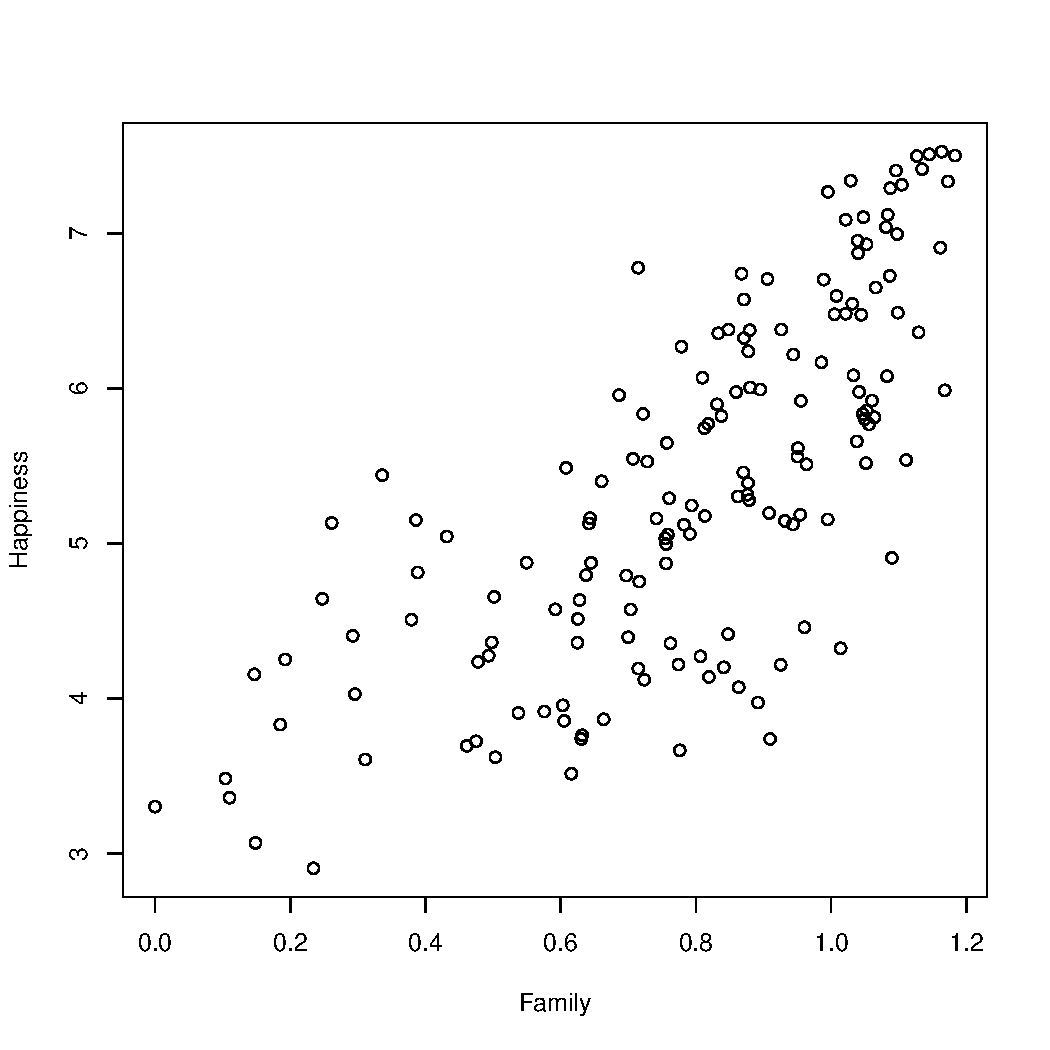
\includegraphics[width=.45\textwidth]{fam_plot.pdf}\hfill
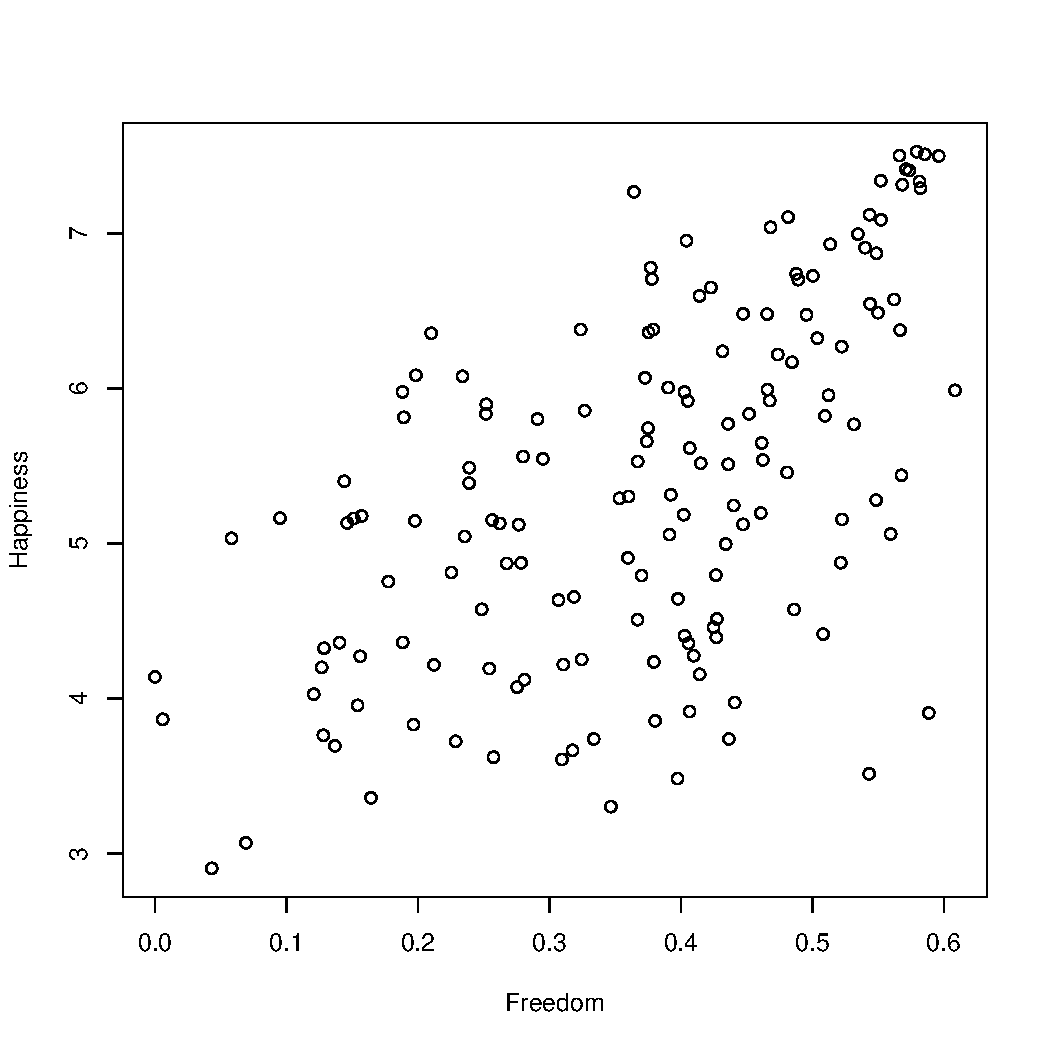
\includegraphics[width=.45\textwidth]{free_plot.pdf}\hfill
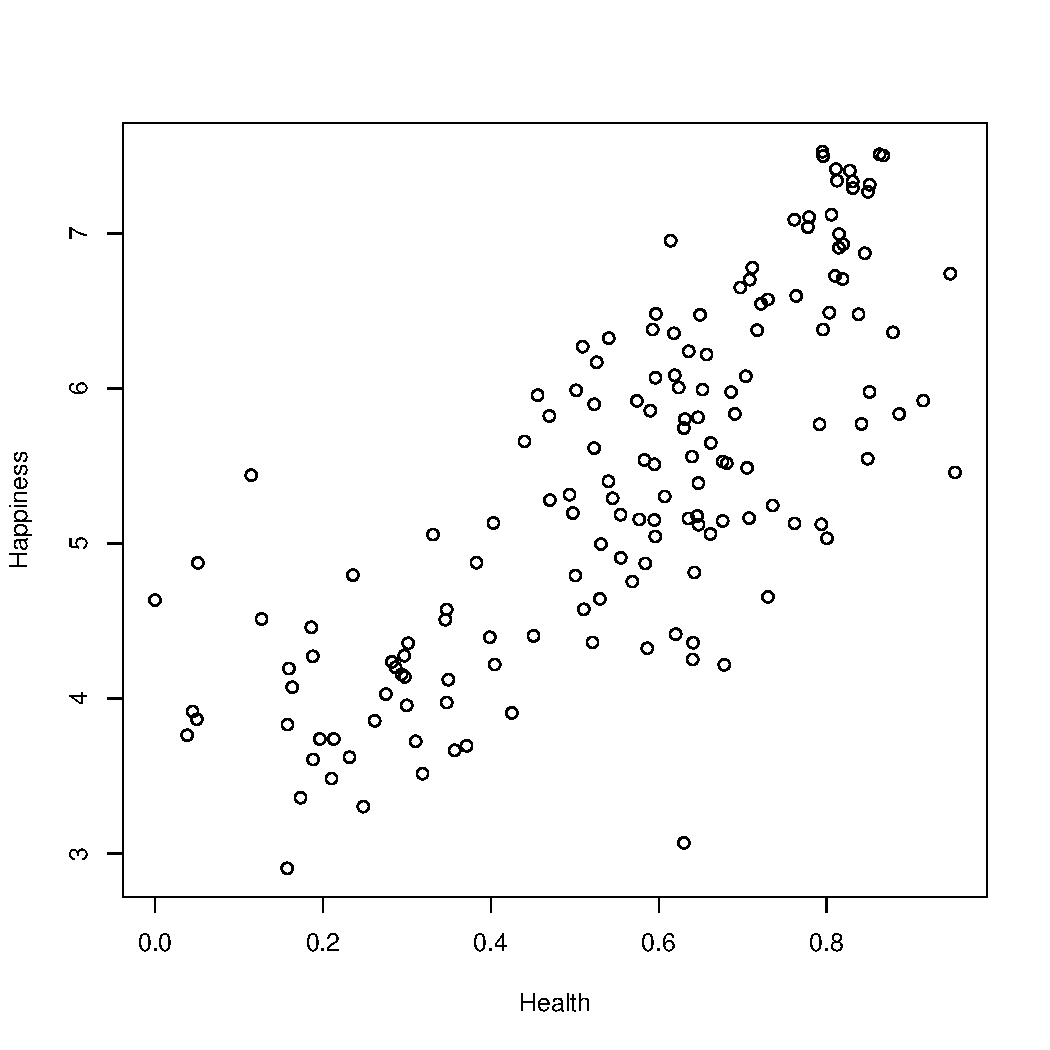
\includegraphics[width=.45\textwidth]{health_plot.pdf}\hfill
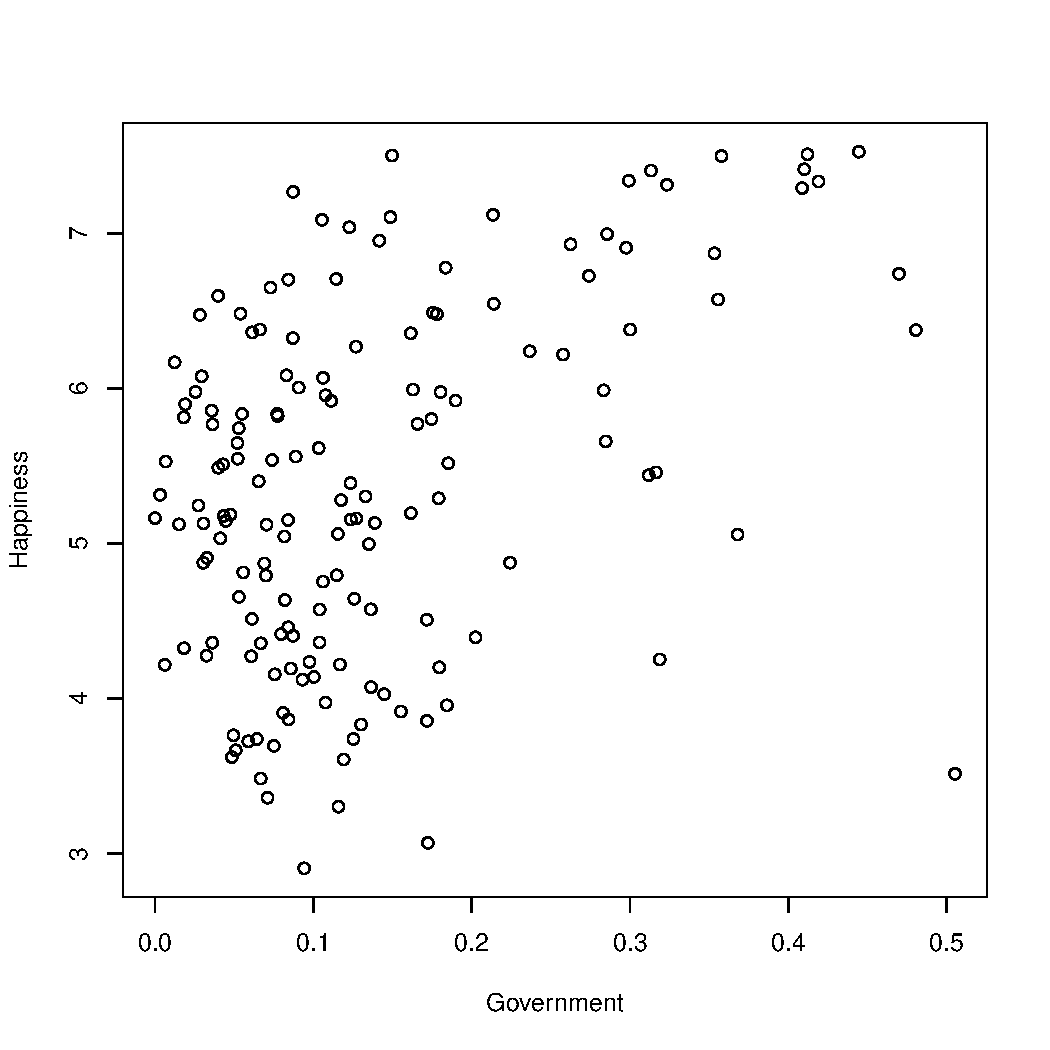
\includegraphics[width=.45\textwidth]{gov_plot.pdf}\hfill

\caption{Scatter Plots}
\label{fig:figure3}

\end{figure}


\end{homeworkProblem}




\end{document}
